\chapter{Models with Time--Varying Dynamics for Pandemic A(H1N1) Influenza in Finland}
\label{chap:lna_extensions}

\section{Overview}
\label{sec:lna_extensions_overview}
To this point, we have largely worked with stochastic epidemic models (SEMs) where the transmission dynamics of an outbreak are taken to be constant over time. This might be only mildly unreasonable for short outbreaks in closed, relatively ``well--mixed" populations, and is often an attractive modeling choice as SEMs with static dynamics are easier to interpret and fit. Incidence data typically arise in settings where the outbreak milieu can change due to environmental changes, heterogeneity in the contact structures of various subpopulations as they are exposed, or behavioral responses as people become aware of an outbreak (or complacent about the extent to which it is under control). Furthermore, we are often interested in understanding the effects of interventions that are time--varying in their implementation or action, such as vaccination campaigns, on the transmission dynamics of an outbreak. Thus, it is important, if not necessary, that we allow the time--varying aspects of an outbreak to be flexibly expressed in the model.

In this chapter, we will use SEMs with time--varying force of infection to model the spread of pandemic A(H1N1) influenza in Finland using surveillance data. Our goals will be to quantify the transmission dynamics of the outbreak, to estimate the true incidence, and to understand what effect a national vaccination campaign had in mitigating the outbreak severity. We will fit several models of varying complexity using the linear noise approximation (LNA) framework developed in Chapter \ref{chap:lna_for_sems}.

\subsection{Pandemic A(H1N1) Influenza in Finland}
\label{subsec:flu_description}

The emergence of a pandemic influenza A strain, A(H1N1)pdm09, in the spring of 2009 led to widespread concern about the potential for high mortality and excessive strain on public health systems around the world. The strain, colloquially referred to as ``swine flu" was a triple reassortment of human, avian, and swine viruses, and was of particular concern because of its similarity with the 1918 pandemic strain that infected up to a third of the world's population and led to an estimated 50 million deaths \cite{cdc1918pandemic}. While the burden imposed by the 2009 pandemic was ultimately comparable to that of seasonal influenza \cite{iuliano2018estimates}, it nevertheless resulted in an estimated 110,000--400,000 respiratory deaths and 50,000--180,000 cardivascular deaths \cite{dawood2012estimated}. The age--standardized cumulative incidence was estimated from serological samples in 19 countries to be between 20\%--27\% \cite{van2013estimating}, with attack rates and transmission dynamics varying greatly by age, and being consistently more severe in children and adolescents \cite{opatowski2011transmission,steens2011age,van2013estimating,yang2015inference}. 

Here, we will analyze surveillance data, displayed in Figure \ref{fig:finland_fludat}, from the first and second waves of the epidemic in Finland. The full dataset, previously analyzed in \cite{shubin2014estimating} and \cite{shubin2016revealing}, consists of weekly laboratory--confirmed A(H1N1) counts, aggregated into sixteen age strata, that were culled from a national surveillance system \cite{lyytikainen2011surveillance}. All cases the data we consider were of mild severity, i.e., cases that did not require hospitalization. Following \cite{shubin2014estimating,shubin2016revealing}, all A(H1N1) cases were treated as A(H1N1)pdm09 due to the high proportion of A(H1N1) cases that were of the pandemic strain. 

An important aspect of the pandemic response in Finland was the execution of a concerted vaccination campaign with the adjuvented monovalent vaccine Pandemrix. Each resident was offered one vaccine dose, free of charge, starting in October, 2009. Vaccination priority was given to health care workers, vulnerable individuals, and young people under the age of 20 \cite{syrjanen2014effectiveness}.  Coverage levels and the timing of vaccination administration varied by age, see Figure \ref{fig:finland_fludat}, with highest coverage among children under the age of 15 ($ \approx $70\%) and the lowest among young adults between the ages of 20--29 ($ \approx $30\%). 

\begin{sidewaysfigure}
	\centering
	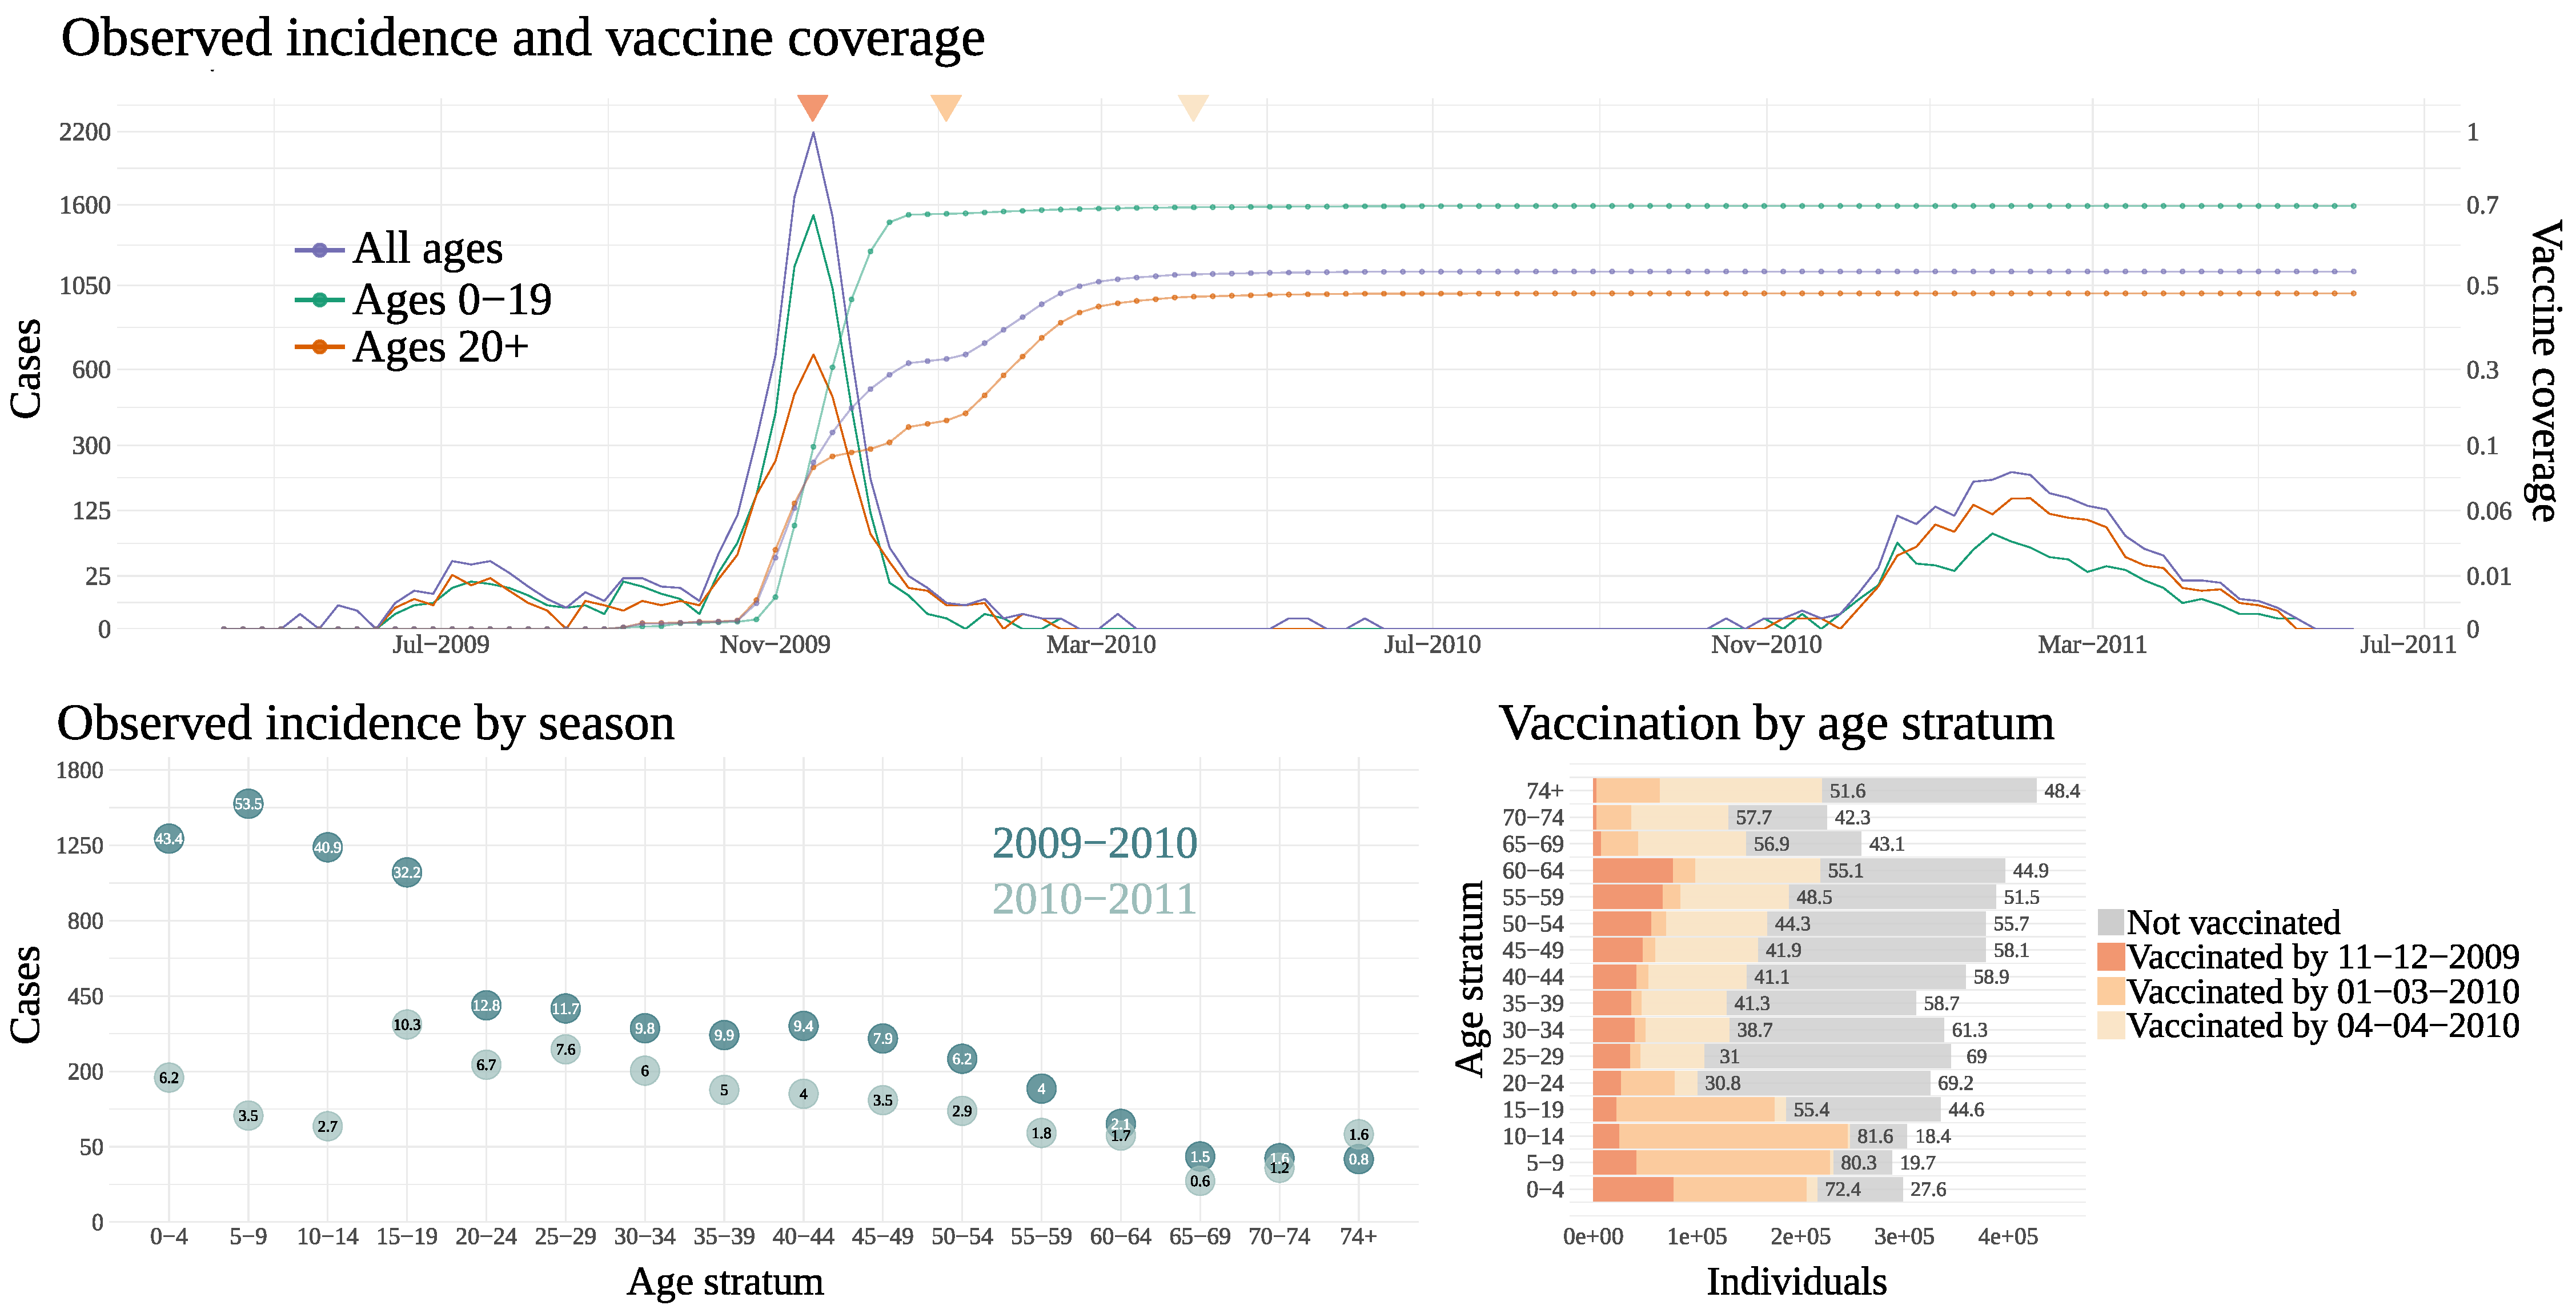
\includegraphics[width=\linewidth]{figures/fludat_plots}
	\caption{(Top) Observed incidence (solid lines) and vaccine coverage (lines with points). (Bottom left) Observed incidence by season and age stratum. The 2009--2010 season (dark green) corresponds to the period from April 15, 2009 through April 4, 2010. The 2010--2011 season (light green) corresponds to the period from September 12, 2010 through June 5, 2011. Numbers in points give the attack rate within each stratum for the corresponding season. (Bottom right) Vaccination coverage by age stratum, colored by vaccine coverages at the times of peak incidence in the first season, tail of the major outbreak in the first season, and end of the vaccination campaign. The numbers inside and outside the histograms denote the percentage of individuals in each stratum that were vaccinated and unvaccinated, respectively, by the end of the vaccination campaign. The times at which vaccine coverages are summarized, denoted by colors of histogram bars, are also identified by corresponding triangles above the top figure.}
	\label{fig:finland_fludat}
\end{sidewaysfigure}


\subsection{The Importance of Allowing for Time--Varying Dynamics}
\label{subsec:tparam_motivation}




\section{Models with Time--Varying Dynamics}
\label{sec:flu_tparam_models}

\subsection{Modeling Time--Varying Force of Infection with a Fixed Functional Form}
\label{subsec:flu_quadfoi}

\subsection{Flexible Models for the Force of Infection with Gaussian Markov Random Fields}
\label{subsec:flu_gmrf}

\subsection{More models}

\section{Discussion}